\documentclass[letterpaper]{article}
    \usepackage{amsmath}
    \usepackage{tikz}
    \usepackage{epigraph}
    \usepackage{lipsum}
    \usepackage{glossaries}
    \usepackage{graphicx}
    \graphicspath{{Images/}}
    \setcounter{tocdepth}{1}
    \makeglossaries
    \renewcommand\epigraphflush{flushright}
    \renewcommand\epigraphsize{\normalsize}
    \setlength\epigraphwidth{0.7\textwidth}

    \definecolor{titlepagecolor}{cmyk}{1,.60,0,.40}

    \DeclareFixedFont{\titlefont}{T1}{ppl}{b}{it}{0.5in}

    \makeatletter
    \def\printauthor{%
        {\large \@author}}
    \makeatother
    \author{
        Brittany Lacy \\
        Drake Lambert \\
        Jeremy LeJeune \\
        Jenna Meadors \\
        Sam Miller \\
       }

    % The following code is borrowed from:  https://tex.stackexchange.com/a/86310/10898

    \newcommand\titlepagedecoration{%
    \begin{tikzpicture}[remember picture,overlay,shorten >= -10pt]

    \coordinate (aux1) at ([yshift=-15pt]current page.north east);
    \coordinate (aux2) at ([yshift=-410pt]current page.north east);
    \coordinate (aux3) at ([xshift=-4.5cm]current page.north east);
    \coordinate (aux4) at ([yshift=-150pt]current page.north east);

    \begin{scope}[titlepagecolor!40,line width=12pt,rounded corners=12pt]
    \draw
      (aux1) -- coordinate (a)
      ++(225:5) --
      ++(-45:5.1) coordinate (b);
    \draw[shorten <= -10pt]
      (aux3) --
      (a) --
      (aux1);
    \draw[opacity=0.6,titlepagecolor,shorten <= -10pt]
      (b) --
      ++(225:2.2) --
      ++(-45:2.2);
    \end{scope}
    \draw[titlepagecolor,line width=8pt,rounded corners=8pt,shorten <= -10pt]
      (aux4) --
      ++(225:0.8) --
      ++(-45:0.8);
    \begin{scope}[titlepagecolor!70,line width=6pt,rounded corners=8pt]
    \draw[shorten <= -10pt]
      (aux2) --
      ++(225:3) coordinate[pos=0.45] (c) --
      ++(-45:3.1);
    \draw
      (aux2) --
      (c) --
      ++(135:2.5) --
      ++(45:2.5) --
      ++(-45:2.5) coordinate[pos=0.3] (d);
    \draw
      (d) -- +(45:1);
    \end{scope}
    \end{tikzpicture}%
    }

\begin{document}
\begin{titlepage}

	\noindent
	\titlefont The Golden Ticket\par
	\epigraph{Software Requirements Document}%
	{\textit{}\\ \textsc{}}
	\null\vfill
	\vspace*{1cm}
	\noindent
	\hfill
	\begin{minipage}{0.35\linewidth}
		\begin{flushright}
			\printauthor
		\end{flushright}
	\end{minipage}
	%
	\begin{minipage}{0.02\linewidth}
		\rule{1pt}{125pt}
	\end{minipage}
	\titlepagedecoration
\end{titlepage}
\tableofcontents
\pagebreak
% This defines the expected readership of the document and describes its version history, including the rationale for the creation of a new version and a summary of the changes made in each version.
\section{Preface}
This document is a complete rewrite of the previously submitted version in order to better fit the format required of the requirements document. This document will contain all of the information of the previous document, and will additionally contain the sections as suggested in the textbook.

Summary of changes: 
\begin{itemize}
	\item One
	\item two
\end{itemize}

In making this document we intend to layout the master plan for a ticketing system using Microsoft's dot net core and the C\# language. This document is intended to be read by anyone intending to create this ticketing system or those intending to use it.
\pagebreak

% This describes the need for the system. It should briefly describe the system's functions and explain how it will work with other systems. It should also describe how the system fits into the overall business or strategic objectives of the organization commissioning the software.
\section{Introduction}
The Golden Ticket is designed to be a lightweight web based ticketing system written using the c\# language. The front end of of the ticketing system will be a responsive designed website so that it is accessible on as many devices as possible. The back-end for the sight will be a micro-services implementation hosted on a debian server featuring sql-lite, the dot net core, identity server 4, lets-encrypt,the apache web server 2.0, and more. The server will feature continuous deployment, when a revision is pushed to the master branch the server will on its check (every minute) download and deploy the change and restart any changes that are needed. In this ticketing system there will be two users of the interface, technicians and admins/managers. This is added text.

\begin{enumerate}
	\item Technicians will have access to the ticket queue and assigned tickets.
	\item Admins will have access to the ticket queue, assigned tickets (if any) and the admin portal.
	\item The ticket queue will consist of all tickets that are not marked as complete. The ticket at the top of the queue will be the ticket whose due date is closest to now / farthest past due. Their will be options to filter views on tickets, such as only tickets assigned to you, only tickets at x difficulty level, etc.
	\item A ticket will consist of the following items:
	      \begin{itemize}
		      \item Title
		      \item Description
		      \item Difficulty level
		      \item A boolean isPriority that can be set by administrators to bring the ticket to the top of the list.
		      \item Contact
		      \item Company/department
		      \item notes + time entries
		      \item assigned technician
		      \item due date/ time
	      \end{itemize}
	\item A contact will consist of the following items:
	      \begin{itemize}
		      \item Name
		      \item Phone number
		      \item Email address
		      \item Title
		      \item Company/department name
	      \end{itemize}
	\item a company will consist of the following items:
	      \begin{itemize}
		      \item A list of contacts
		      \item A list of associated tickets
		      \item join date
	      \end{itemize}
  \item A Technician will consist of the following items:
        \begin{itemize}
          \item Join date
          \item experience level
          \item Email
          \item phone
          \item list of assigned tickets
        \end{itemize}
  \item An administrator will consist of the following items:
        \begin{itemize}
          \item 
        \end{itemize}
\end{enumerate}
\pagebreak

% This defines the technical terms used in the document. You should not make assumptions about the experiences or expertise of the reader.
\section{Glossary}
\pagebreak

% Here, you describe the services provided for the user. The nonfunctional system requirements should also be described in this section. This description may use natural language, diagrams, or other notations that are understandable to customers. Product and process standards that must be followed should be specified.
\section{User Requirements definition}
\pagebreak

% This chapter presents a high-level overview of the anticipated system architecture, showing the distribution of functions across system modules. Architectural components that are reused should be highlighted.
\section{System Architecture}
\begin{figure}[htbp]
  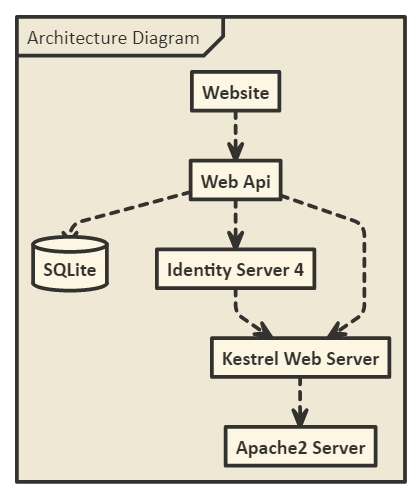
\includegraphics[scale = .5]{ArchitectureDiagram.png}
  \caption{Architecture Diagram}[The diagram describing the architecture of the system]
  \centering
\end{figure}
The above figure describes the main processes and applications that will be used to run this system.

\begin{figure}[htbp]
  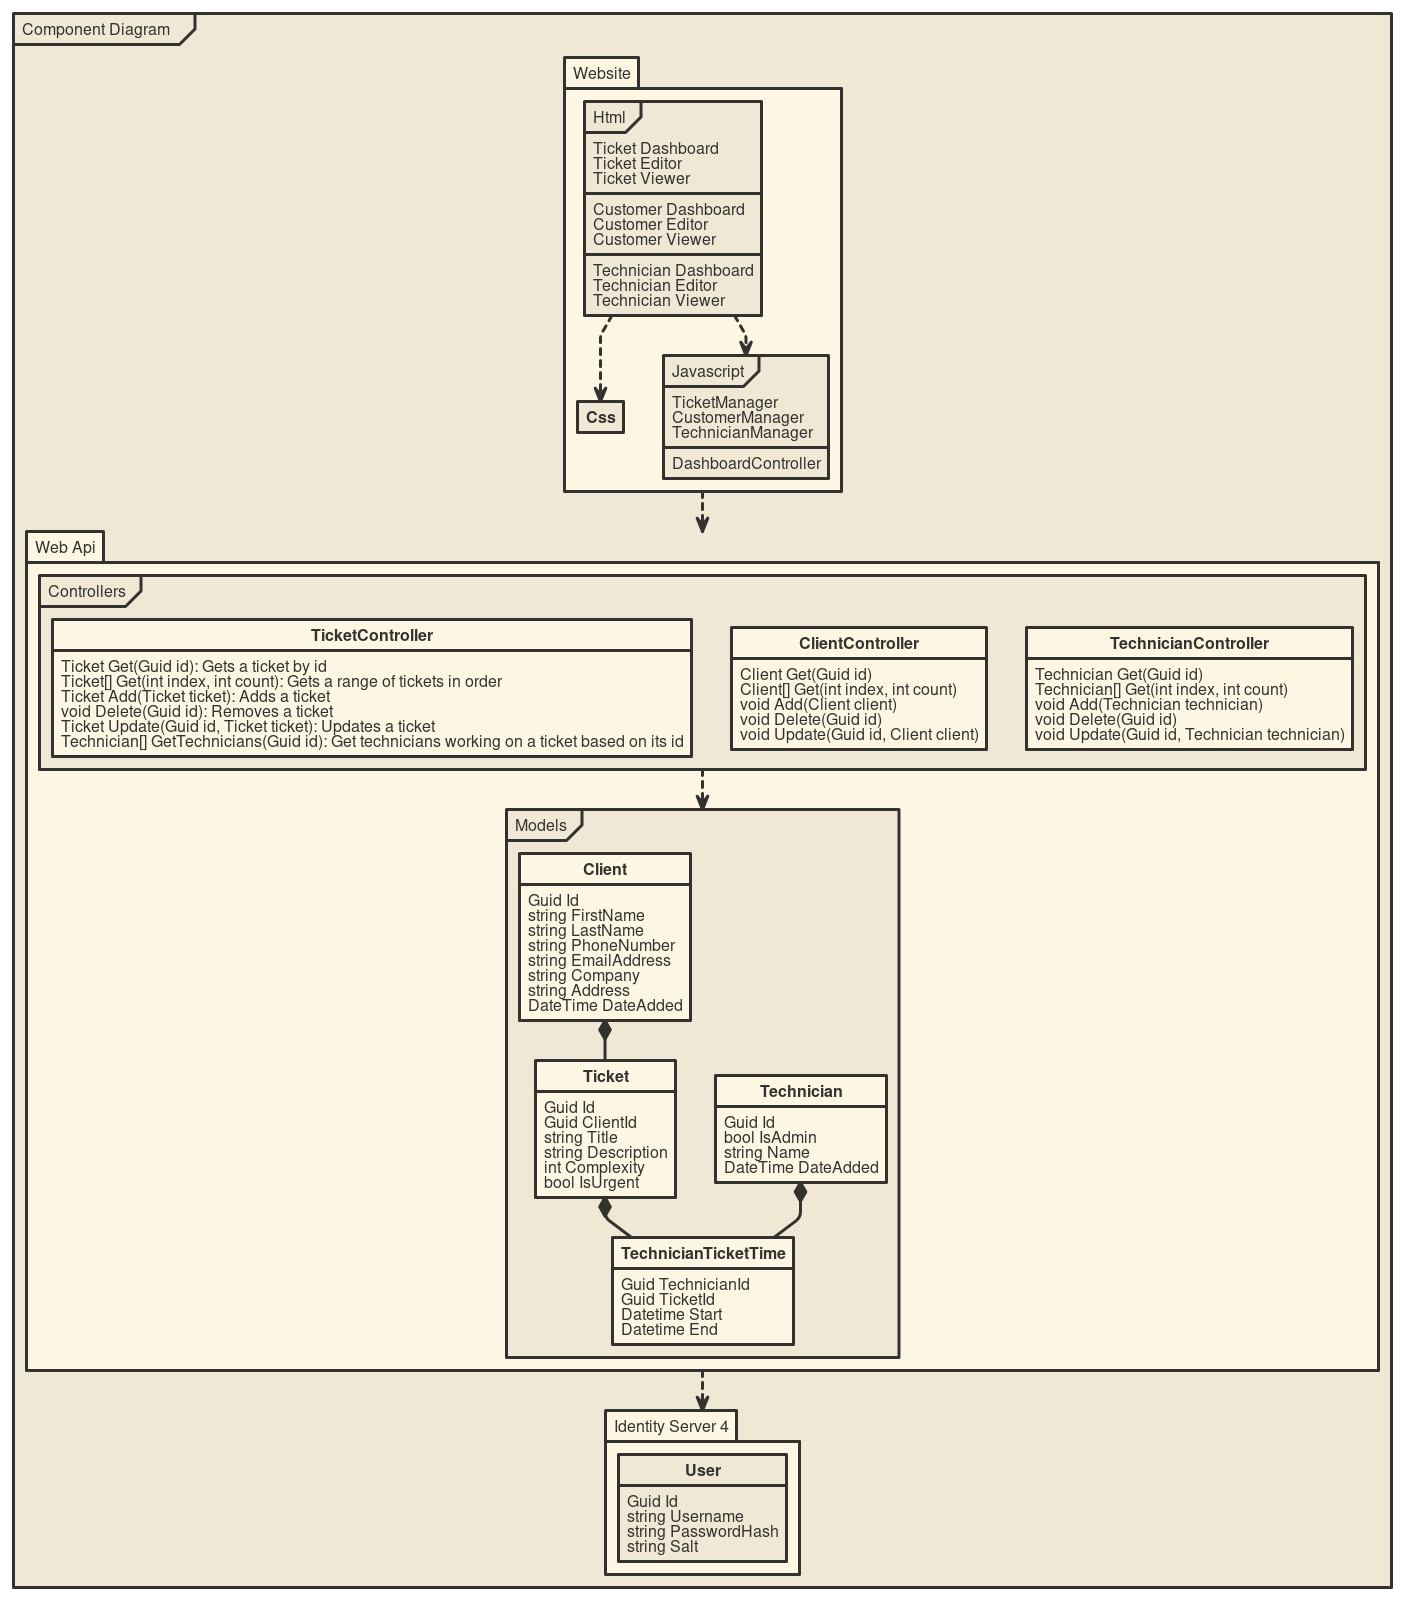
\includegraphics[scale =.5, width = \textwidth, height = \textheight]{ComponentDiagram.png}
  \caption{Component Diagram}[The diagram describing the components and classes of the system]
  \centering
\end{figure}
\pagebreak

% This describes the functional and nonfunctional requirements in more detail. If necessary, further detail may also be added to the nonfunctional requirements. Interfaces to other systems may be defined.
\section{System Requirements Specification}
\pagebreak

% This chapter includes graphical system models showing the relationships between the system components and the system and its environment. Examples of possible models are object models, data-flow models, or semantic data models.
\section{System Models}
\pagebreak

% This describes the fundamental assumptions on which the system is based, and any anticipated changes due to hardware evolution, changing user needs, and so on. This section is useful for system designers as it may help them avoid design decisions that would constrain likely future changes to the system.
\section{System Evolution}
\pagebreak

% These provide detailed, specific information that is related to the application being developed—for example, hardware and database descriptions. Hardware requirements define the minimal and optimal configurations for the system. Database requirements define the logical organization of the data used by the system and the relationships between data.
\section{Appendices}
\pagebreak

% Several indexes to the document may be included. As well as a normal alphabetic index, there may be an index of diagrams, an index of functions, and so on.
\section{Index}

\listoffigures
\pagebreak



\end{document}
